\documentclass[tikz,border=5pt]{standalone}
\usepackage{amssymb,amsmath}
\usepackage{tikz}
\usepackage{lmodern}
\usetikzlibrary{calc}

\begin{document}

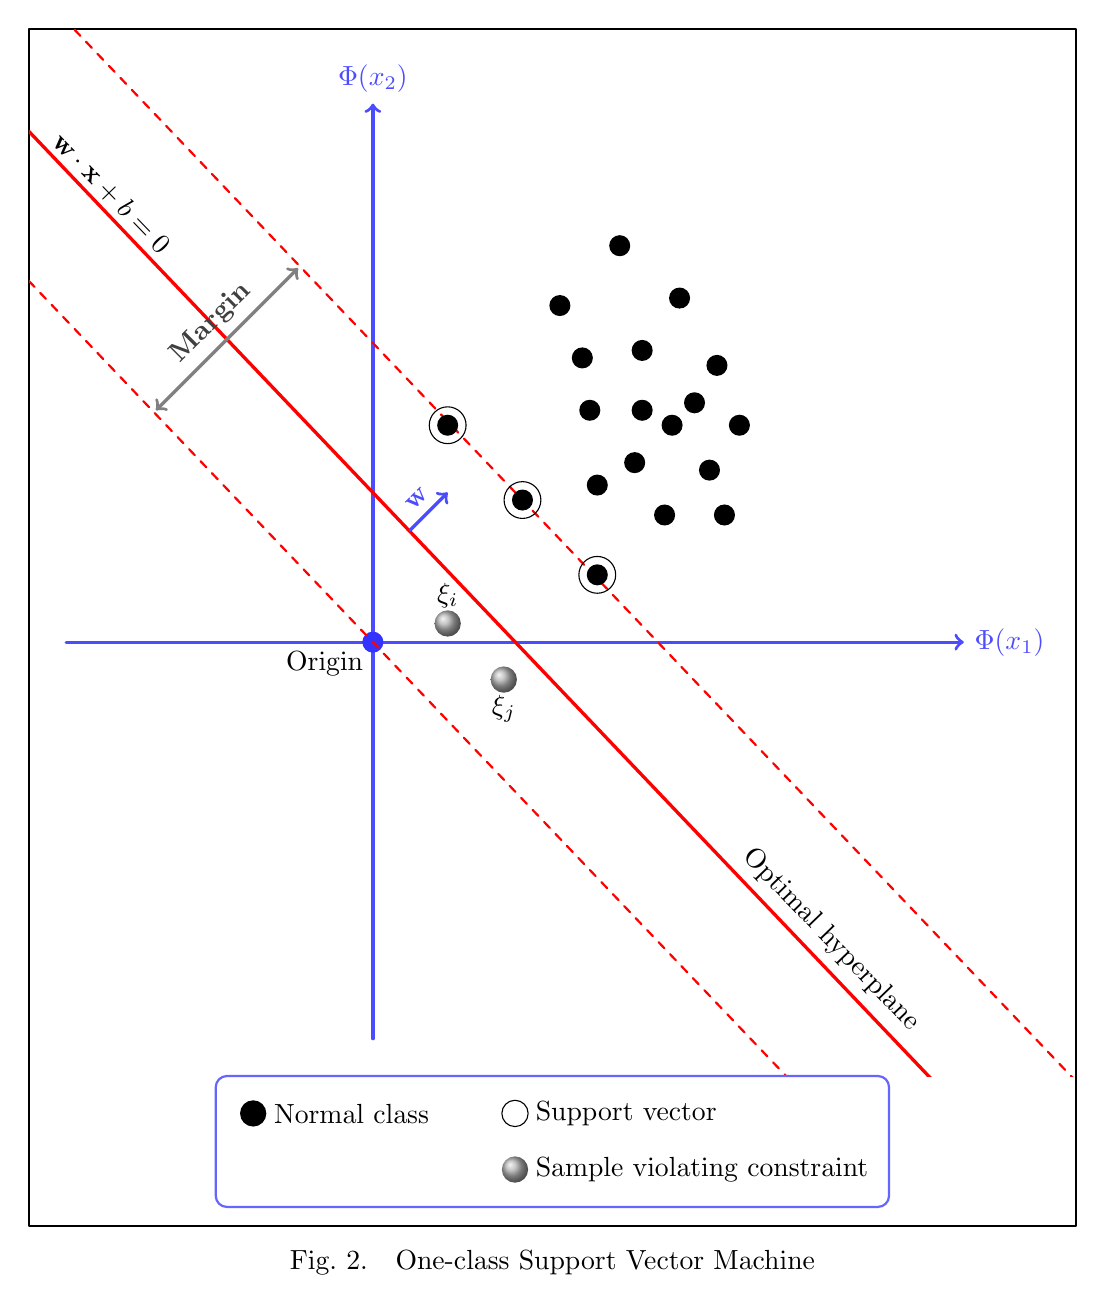
\begin{tikzpicture}[scale=0.95, line cap=round, line join=round]
	
	% ----------------------------
	% 0) Canvas box
	% ----------------------------
	\def\xmin{-7} \def\xmax{7}
	\def\ymin{-7} \def\ymax{7}
	\draw[thick] (\xmin,\ymin-2) rectangle (\xmax,\ymax);
	
	% ----------------------------
	% 1) Off-center origin (like the figure)
	% ----------------------------
	\def\Ox{-2.4}
	\def\Oy{-1.2}
	\coordinate (O) at (\Ox,\Oy);
	
	\begin{scope}
		\clip (\xmin,\ymin) rectangle (\xmax,\ymax);
		
		% ----------------------------
		% 2) Axes
		% ----------------------------
		\draw[blue!70, very thick, ->] (\xmin+0.5,\Oy) -- (\xmax-1.5,\Oy)
		node[right] {$\Phi(x_1)$};
		\draw[blue!70, very thick, ->] (\Ox,\ymin+0.5) -- (\Ox,\ymax-1)
		node[above] {$\Phi(x_2)$};
		
		\fill[blue!80] (O) circle (4pt);
		\node[below left] at (O) {Origin};
		
		% ----------------------------
		% 3) Hyperplane + two margins (parallel)
		%    y - Oy = m(x - Ox) + c
		% ----------------------------
		\def\m{-1.05}   % slope
		\def\c{2.0}     % shift
		\def\dm{2}    % margin spacing
		
		% solid hyperplane
		\draw[red, very thick]
		(\xmin,{ \Oy + \m*(\xmin-\Ox) + \c }) --
		(\xmax,{ \Oy + \m*(\xmax-\Ox) + \c })
		node[pos=0.75, rotate=-46, black, above] {Optimal hyperplane};
		
		% dashed margins
		\draw[red, dashed, thick]
		(\xmin,{ \Oy + \m*(\xmin-\Ox) + \c + \dm }) --
		(\xmax,{ \Oy + \m*(\xmax-\Ox) + \c + \dm });
		
		\draw[red, dashed, thick]
		(\xmin,{ \Oy + \m*(\xmin-\Ox) + \c - \dm }) --
		(\xmax,{ \Oy + \m*(\xmax-\Ox) + \c - \dm });
		
		\node[rotate=-46] at (\Ox-3.5,\Oy+6.0) {$\textbf{w}\cdot \textbf{x} + b = 0$};
		
		% ----------------------------
		% 4) Margin arrow
		% ----------------------------
		\draw[gray, very thick, <->] (\Ox-1,\Oy+5) -- (\Ox-2.9,\Oy+3.1) node[gray!50!black, sloped, above, midway, font=\bfseries] {Margin};
		
		% ----------------------------
		% 5) w arrow
		% ----------------------------
		\draw[blue!70, very thick, ->] (\Ox+.5,\Oy+1.5) -- (\Ox+1,\Oy+2) node[sloped, above, midway] {$\textbf{w}$};
		
		% ----------------------------
		% 6) Normal class points (black cluster)
		% ----------------------------
		\foreach \p in {
			(0.9,4.1),(0.1,3.3),(1.7,3.4),(1.2,2.7),(0.4,2.6),
			(2.2,2.5),(0.5,1.9),(1.6,1.7),(2.5,1.7),(1.1,1.2),
			(2.1,1.1),(0.6,0.9),(1.5,0.5),(2.3,0.5),
			(1.2,1.9),(1.9,2.0)
		}{
			\fill \p circle (4pt);
		}
		
		% ----------------------------
		% 7) Support vectors (circled points)
		% ----------------------------
		\foreach \p in {(\Ox+2,\Oy+1.9), (\Ox+1,\Oy+2.9), (\Ox+3,\Oy+.9)}{
			\fill \p circle (4pt);
			\draw \p circle (7pt);
		}
		
		% ----------------------------
		% 8) Samples violating constraint (gray balls) + xi labels
		% ----------------------------
		\shade[ball color=gray!60] (\Ox+1,\Oy+.25) circle (5pt) node[above=2pt] {$\xi_i$};
		\shade[ball color=gray!60] (\Ox+1.75,\Oy-.5) circle (5pt) node[below=2pt] {$\xi_j$};
	\end{scope}
	
	% ----------------------------
	% 9) Legend box
	% ----------------------------
	\begin{scope}[shift={(0,-8)}]
		\draw[blue!60, fill=white, thick, rounded corners=4pt] (-4.5,-.75) rectangle (4.5,1.0);
		
		\fill (-4,0.5) circle (5pt) node[right=4pt] {Normal class};
		\draw (-.5,.5) circle (5pt) node[right=4pt] {Support vector};
		\shade[ball color=gray!60] (-.5,-0.25) circle (5pt) node[right=4pt] {Sample violating constraint};
	\end{scope}
	
	% ----------------------------
	% 10) Caption (optional)
	% ----------------------------
	\node at (0,-9.5) {Fig.\ 2.\quad One-class Support Vector Machine};
	
\end{tikzpicture}
\end{document}